\section{Introduction}
\begin{wrapfigure}[14]{r}{0.48\textwidth}
\begin{center}
\vspace{-40pt}
    \centering
    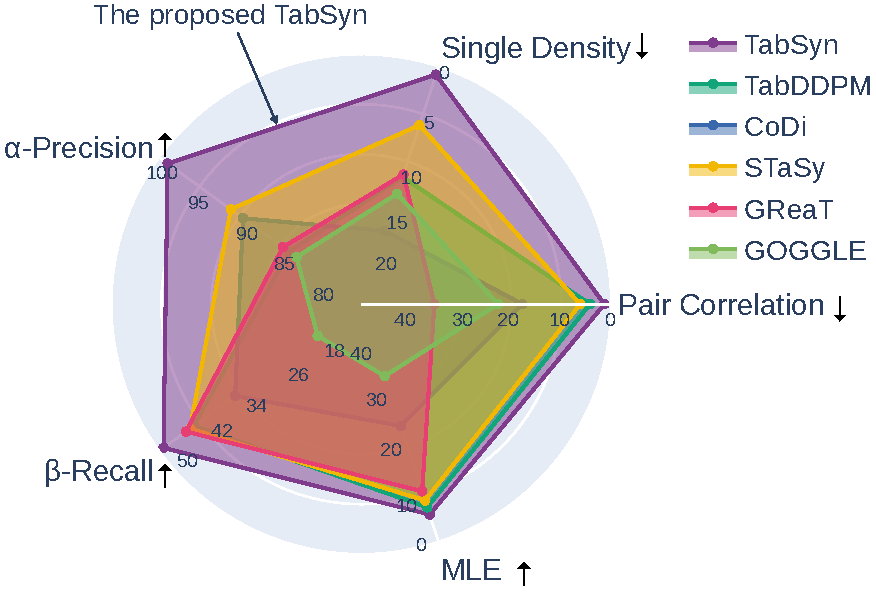
\includegraphics[width = 1.0\linewidth]{Fig/radar.pdf}
    \caption{Our \modelname consistently outperforms SOTA tabular data generation methods across five data quality metrics.
    }
    \label{fig:radar}
\end{center}
\end{wrapfigure}

Tabular data synthesis has a wide range of applications, such as augmenting training data~\citep{fonseca2023tabular}, protecting private data instances~\citep{privacy, privacy_health}, and imputing missing values~\citep{TabCSDI}.
Recent developments in tabular data generation have notably enhanced the quality of synthetic data~\citep{ctgan, great, goggle}, while the synthetic data is still far from the real one. To further improve the generation quality, researchers have explored adapting diffusion models, which have shown strong performance in image synthesis tasks~\citep{ddpm, ldm}, for tabular data generation~\citep{sos, tabddpm, stasy, codi}. Despite the progress made by these methods, tailoring a diffusion model for tabular data leads to several challenges. Unlike image data, which comprises pure continuous pixel values with local spatial correlations, tabular data features have complex and varied distributions~\citep{ctgan}, making it hard to learn joint probabilities across multiple columns. Moreover, typical tabular data often contains mixed data types, i.e., continuous (e.g., numerical features) and discrete (e.g., categorical features) variables. The standard diffusion process assumes a continuous input space with Gaussian noise perturbation, which leads to additional challenges with categorical features. Existing solutions either transform categorical features into numerical ones using techniques like one-hot encoding~\citep{stasy, goggle} and analog bit encoding~\citep{TabCSDI} or resort to two separate diffusion processes for numerical and categorical features~\citep{tabddpm, codi}. However, it has been proven that simple encoding methods lead to suboptimal 
performance~\citep{codi}, and learning separate models for different data types makes it challenging for the model to capture the co-occurrence patterns of different types of data. Therefore, we seek to develop a diffusion model in a joint space of numerical and categorical features that preserves the inter-column correlations.

This paper presents \emph{\modelname{}}, a principled approach for tabular data synthesis. To handle mixed-typed inputs, \modelname first transforms raw tabular data into a continuous embedding space, where well-developed diffusion models with Gaussian noises become feasible. Subsequently, we learn a score-based diffusion model in the embedding space to capture the distribution of latent embeddings. To learn an informative, smoothed latent space while maintaining the decoder's reconstruction ability, we specifically designed a Variational AutoEncoder (VAE~\citep{vae}) model for tabular-structured data. Our proposed VAE model includes 1) Transformer-architecture encoders and decoders for modeling inter-column relationships and obtaining token-level representations, facilitating token-level tasks. 2) Adaptive loss weighting to dynamically adjust the reconstruction loss weights and KL-divergence weights, allowing the model to improve reconstruction performance gradually while maintaining a regularized embedding space. 3) Finally, when applying diffusion models in the latent space, we adopt a simplified forward diffusion process, which adds Gaussian noises of linear standard deviation with respect to time. We demonstrate through theoretical analysis and empirical justifications that this approach can reduce the errors in the reverse process, thus improving sampling speed. 

The advantages of \modelname are three-fold: 
(1) \generality: \textit{Mixed-type Feature Handling} - \modelname transforms diverse input features, encompassing numerical, categorical, etc., into a unified embedding space.
(2) \quality: \textit{High Generation Quality} - with tailored designs of the VAE model, the tabular data is mapped into regularized latent space of good shape, e.g., a standard normal distribution. This will greatly simplify training the subsequent diffusion model~\citep{sgm}, making \modelname more expressive and enabling it to generate high-quality synthetic data. 
(3) \speed: 
With the proposed linear noise schedule, our \modelname can generate high-quality synthetic data with fewer than $20$ reverse steps, which is significantly fewer than existing methods.

Recognizing the absence of unified and comprehensive evaluations for synthetic tabular data~\citep{assess}, we perform extensive experiments, which involve comparing \modelname with seven state-of-the-art methods on six mixed-type tabular datasets using over five distinct evaluation metrics.
The experimental results demonstrate that \modelname consistently outperforms previous methods (see Figure \ref{fig:radar}). Specifically, \modelname reduces the average errors in column-wise distribution shape estimation (i.e., single density) and pair-wise column correlation estimation (i.e., pair correlation) tasks by $86\%$ and $67\%$ than the most competitive baselines. Furthermore, we demonstrate that \modelname achieves competitive performance across two downstream tabular data tasks, machine learning efficiency and missing value imputation. Specifically, the well-learned unconditional \modelname is able to be applied to missing value imputation without retraining. Moreover, thorough ablation studies and visualization case studies substantiate the rationale and effectiveness of our developed approach.
